\chapter{Testing and Verification}
\label{app:testing}

This appendix summarises how the data and the simulator were checked. No amount of
testing proves a program has no errors; it can only make specific errors hard to
miss. Two independent test systems back the engines and the metrics: a suite of
\VerTestsTotal\ automatic Rust tests (\VerTestsPassed\ pass; \VerTestsIgnored\ need
real data or system tools and run separately), and a checklist of
\VerChecklistTotal\ hand-worked scenarios (\VerChecklistCda\ CDA, \VerChecklistFba\
FBA, \VerChecklistMet\ metrics) compiled into the simulator itself, so it runs on the
finished executable with no development tools. On top of these, three further checks
were built specifically for this appendix: an independent second implementation of
both engines, deliberately planted bugs to confirm the tests can actually catch
mistakes, and a comparison of the simulated output with what really happened on the
venue. All numbers below come from the scripts listed in \Cref{sec:testlimits}, run
on the full December~2025 data and result files.

\section{The Input Data}
\label{sec:testdata}
\label{sec:testfiles}

The 54-byte binary format is decoded by dedicated unit tests, including one that
decodes the literal bytes of a real record and checks every field against the
value printed in the dataset's own preview file. Because unit tests on a few
records cannot show that all \VerRecords\ are read correctly, the whole archive was
decoded a second time by an independent program that shares no code with the
simulator. \Cref{tab:testcounts} compares its counts
with the simulator's own \texttt{scan} command and its running totals: all three
agree exactly, and the four record categories add up to the total with no remainder.

\begin{table}[htbp]
\centering
\caption[Independent record counts]{Record counts for the December 2025 SOL
archive from three independent programs.}
\label{tab:testcounts}
\small
\begin{tabularx}{\textwidth}{@{}L r r r@{}}
\toprule
\textbf{Quantity} & \textbf{Scan command} & \textbf{Simulation} & \textbf{Second decoder}\\
\midrule
Hourly files read & 744 & 744 & \VerFiles\\
Total records & 640,176,812 & 640,176,812 & \VerRecords\\
New live orders & 283,797,135 & --- & \VerNewLive\\
Cancellations & 281,778,306 & --- & \VerCancels\\
Other records (fills, rejections, \dots) & 57,615,417 & --- & \VerOther\\
Size rounds to zero (skipped) & 16,985,954 & 16,985,954 & \VerRoundZero\\
\bottomrule
\end{tabularx}
\end{table}

The second decoder also checked ten structural conditions across every file and
record --- file sizes, boolean fields, status/type/time-in-force codes, size
ordering, and timestamp order --- and found none violated. Three smaller
imperfections in the data itself are worth noting, since they affect the results in
small ways discussed later: \VerBackwardTotal\ records have an earlier timestamp
than the one before them (by up to \VerMaxBackwardSec\,s, counted by the replay as
late events, \VerLateCda\ of them for the CDA); \VerGapsTotal\ silences longer than a
minute occur, the longest \VerMaxGapMin\ minutes; and \VerDupPct\ percent of records
(\VerDupRepeats) are byte-for-byte repeats of an earlier record in the same file,
concentrated in a few hours. A repeated \texttt{open} record puts a second copy of
the same order into the replay, which is the reason a handful of one-second buckets
later show a fill rate above one.

Sorting every record by order number and replaying each order's own history checks
that it is opened once, never grows in size, and (with one exception in 60,378
orders, all but one of them conditional orders) has one consistent submission time
throughout. A short section of the dataset's own preview file, with real trades from
the first three seconds of the month, was traced back into the order-status records
by hand and confirms how fills are recorded: 28.14 of 28.26\,SOL of real trades are
recovered this way (the rest is one order that never appears in the archive at all).

\section{The Engines}
\label{sec:testfba}

Both engines were checked three ways. First, a randomised property test: a seeded
stream of orders and cancellations runs through the real engine and, in parallel,
through a deliberately naive reference (a full scan of every resting order for the
CDA; a brute-force scan of every possible price for the FBA), compared after every
event or clearing. This covered 360,000 CDA events across 3,000 scenarios (book
never crossed, every trade at the resting order's price, no order filled beyond its
size) and 36,000 FBA clearings (the price chosen always the true volume-maximiser
among \emph{every} possible price, with the allocation following price-time
priority exactly on both sides). That priority walk is also what confirms a claim
made in \Cref{sec:clearing}: a better-priced order is only ever left partly filled
on the longer side, and only when the volume-maximising price range spans more
than one price --- never on the shorter side, and never when a single price
maximises volume.

Second, \VerChecklistCda\ and \VerChecklistFba\ scenarios worked out by hand cover
the ordinary cases (a plain cross, a multi-level sweep, ties with and without price
history) and the edge cases that are easy to get wrong (an empty book or batch, a
market order with no liquidity, a cancel of an unknown order, roll-over of a
leftover); three are regression tests for real defects found while building the
simulator.

Third, an independent Python re-implementation of both engines (sharing no code or
data structures with the Rust one, decoding the raw records itself) was run against
four full hours of real data: the sample hour, a quiet night, the busiest hour of
the month, and an hour with many repeated records. \Cref{tab:reftable} shows every
prediction it made --- trades, volumes, prices, depths, and for the FBA the
unexecuted share --- matched the Rust output in all \VerRefBuckets\ one-second
buckets checked.

\begin{table}[htbp]
\centering
\caption[Rust engines against an independent reference]{Agreement between an
independently written reference implementation and the Rust simulator, four full
hours. \VerRefMismatches\ disagreements across \VerRefBuckets\ engine-buckets.}
\label{tab:reftable}
\small
\begin{tabularx}{\textwidth}{@{}L r r@{}}
\toprule
\textbf{Hour} & \textbf{Records} & \textbf{Agreement}\\
\midrule
1 Dec, \texttt{sol\_12} & 1,219,826 & every bucket, both engines\\
25 Dec, \texttt{sol\_04} & 294,268 & every bucket, both engines\\
15 Dec, \texttt{sol\_14} & 2,623,879 & every bucket, both engines\\
20 Dec, \texttt{sol\_09} & 387,906 & every bucket, both engines\\
\bottomrule
\end{tabularx}
\end{table}

Finally, to check the tests themselves are strict enough to matter, 19 realistic
bugs were planted one at a time in a copy of the source (never the real engines) ---
e.g.\ changing the CDA's crossing rule from ``at or above'' to ``strictly above'', or
the FBA's tie-break to prefer the larger imbalance instead of the smaller one.
\VerMutSummary

\section{The Metrics and the Result Files}
\label{sec:testmetrics}
\label{sec:testoutputs}

\VerMetricTests\ unit tests check individual metric formulas against numbers worked
out by hand, including recovering an artificially planted Kyle's-lambda slope to
nine decimal places, and confirming that streaming the output file in pieces (as the
real run does) gives byte-identical results to writing it all at once. A further
eight checklist scenarios drive the metrics code with synthetic events and compare
every output column with a hand-computed value. The independent reference
implementation above adds a third, larger-scale check: it recomputes six metrics
(quoted spread, depth, effective spread, unexecuted share) from scratch for every
second of the same four hours, and matches (\Cref{tab:reftable}).

The two month-long result files were then checked for internal consistency: every
relation that follows from a metric's own definition (for example, that price
impact equals effective spread minus realized spread, that a spread is never
negative, that VWAP times volume equals notional) was tested on all \VerRows\ rows
of both files. Of dozens of such relations, only two are ever violated, and both are
understood rather than being errors: the FBA's price dispersion, which should be
exactly zero, is not in \VerDispRows\ buckets where two separate batches happened to
contribute a trade to the same second; and the fill rate, which should never exceed
one, does so in six rows out of \VerFillRows, all traceable to the repeated input
records noted above. Recomputing eleven columns independently from the raw CSV
files, rather than trusting the simulator's own running summary, matched to a
relative error of at most $10^{-8}$ in every case but one (the FBA's Kyle's lambda,
$2.4\times10^{-4}$, a sum of near-cancelling values). Every number quoted anywhere in
this thesis is generated the same way, by a script that also checks that no macro is
left undefined and no cross-reference is left dangling; this process caught and
corrected one real error, a wrongly based percentage of skipped records.

\section{Determinism}
\label{sec:testdeterminism}

The engines contain no random numbers and no clock, so the same input should always
give the same output. Replaying the sample hour twice from scratch, and separately
replaying \VerDetReplays\ random flows through the property tests twice each,
confirms this: of the 35 output columns, 33 are byte-identical between the two runs.
The two that are not, throughput and clearing latency, are measured wall-clock
timings and are labelled as controls for that reason, not as results. This
guarantee applies to an \emph{uninterrupted} run; \Cref{sec:testresets} shows the
month-long run was not one.

\section{Does the Replay Match the Real Venue?}
\label{sec:testfidelity}

Everything above shows the engines do what their rules say. A different question is
whether those rules, applied to the real order flow, give a realistic picture of
what actually happened on the venue --- and the answer is only partly yes. The
archive itself contains the venue's own record of every taker fill (an order filled
the moment it was submitted), so the venue's true traded volume can be measured
directly from data the simulator never even reads. Over the month this comes to
\VerVenueVol\ million SOL, while the simulated volume is \VerCdaVol\ million for the
CDA and \VerFbaVol\ million for the FBA --- about twice as much. The two track each
other closely in time (correlated at \VerCorrDay\ per day) but not in level.

The reason is that the replay does not enforce two rules the real venue does: an
order marked ``post-only'' can never trade as a taker on the real venue, and
self-trades are prevented there but not here. Measuring these directly on a random
sample of 24 whole hours shows that \VerHoursPostPct\ percent of the simulated
volume comes from post-only takers and \VerHoursSelfPct\ percent from a participant
trading with themselves; removing the post-only volume brings the simulated total to
within a few percent of the venue's (\VerHoursExRatio\ times it, against
\VerHoursRatio\ times before). Both engines share this same imperfect input equally,
so the paired comparison between them in \Cref{ch:results} is unaffected, but the
absolute levels of volume and everything computed from it describe the replayed
flow, not the venue exactly. This is the largest limitation this verification found.

\subsection{Does the Price Still Track the Real Market?}
\label{sec:testprice}

The volume mismatch above is about \emph{how much} trades; it says nothing about
\emph{at what price}. Comparing each engine's hourly volume-weighted price against
real hourly SOL-USD candles from Yahoo Finance (\Cref{fig:pricevsyahoo}) shows the
simulated price tracks the real one closely all month: a mean absolute difference of
about \VerPriceMadCda\ bps for the CDA and \VerPriceMadFba\ bps for the FBA, roughly
0.1\% of the price, with the simulated price falling inside that hour's real
trading range \VerPriceInsideCda/\VerPriceInsideFba\ percent of the time. The two
engines differ from each other by only \VerPriceCdaFba\ bps on average, so this small
gap to the real market is a property of the replay, not a difference between the
mechanisms being compared.

\begin{figure}[htbp]
\centering
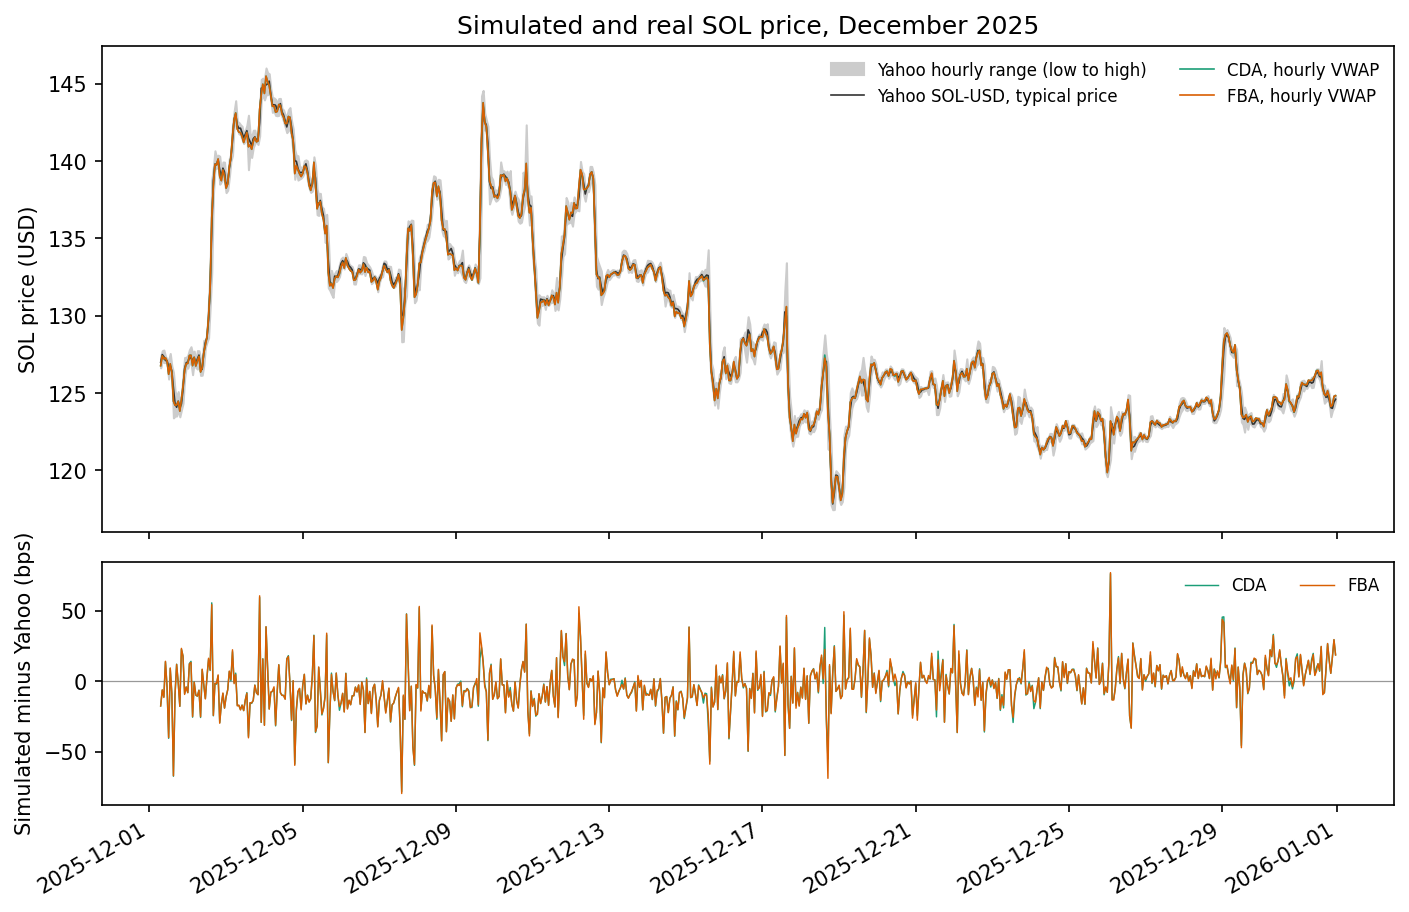
\includegraphics[width=0.95\textwidth]{figures/fig_pricevsyahoo.png}
\caption[Simulated price against the real price]{Hourly volume-weighted price of
each engine against the real SOL-USD price (Yahoo Finance), whole month. Bottom:
simulated minus real price, in basis points.}
\label{fig:pricevsyahoo}
\end{figure}

\section{Was the Month One Continuous Run?}
\label{sec:testresets}

The simulator can save a checkpoint and resume a stopped run, but the code that
resumes creates both engines again from empty, losing every resting or pending
order. This leaves a visible trace: the CDA's book depth briefly collapses at the
start of an hour, and the FBA occasionally clears a batch already split across the
timing grid. Looking for this trace shows \VerResetN\ such restarts, all in the
first five days of the month and none afterward.

Because both engines restart at the same record, the paired comparison between them
is affected equally; but book-state measures, especially CDA depth, are understated
for some hours afterward, and the FBA's batch clock stays briefly out of step with
the metrics grid, which is why its price dispersion is not exactly zero in
\VerDispRows\ buckets. An uninterrupted replay of the month would remove this; this
work did not run one.

\section{What Was Not Checked}
\label{sec:testlimits}

Three things fall outside this verification. The convergence of the FBA to the CDA
as $\tau \to 0$ was not tested, since it needs a sweep over several interval widths
that this thesis does not include. The full month was not replayed by the
independent Python reference, only four hours in detail and 24 more for volume,
because it is far slower than the Rust simulator. And the repeated records and data
silences noted above were measured but not corrected in the results.

Everything here can be reproduced: \texttt{cargo test} runs the automatic tests,
\texttt{market\_sim test engine all} the checklist, and the verification scripts
described above reproduce every number in this appendix.
